\section{Services used}
Hosting service used and why.

Rendering mode used and why.

\section{Structure}
Structure of links/pages folder with short description

As for the structure of the project main folders, we referenced the Nuxt3 standard: the most external index file 
contains the code of the homepage, while each page code is inside its own folder, with the same organization used for navigation.
For the pages of the single Service, Project and Person we used 'slug' .....
In order to maintain the same layout throughout the website we have also utilized layouts: a default one with header (navigation bar), body (page content) and footer;
and a 'no-footer' layout, that we used for the chatbot page specifically.


\begin{center}
    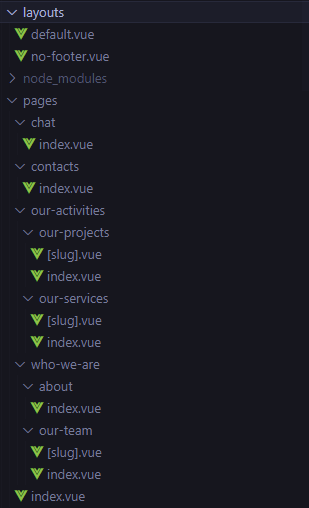
\includegraphics[width=0.25\linewidth]{img/folders-structure.png}
    \captionof{figure}{Pages and layouts folders structure}
\end{center}

\vspace{1em}
Available server endpoint with short description

\section{Components}
List of components implemented with description, props and emit (if used)

Here we describe each of the components we implemented in our project:
\begin{itemize}
    \item App:
    \begin{itemize}
        \item \textbf{AppFooter}: the footer present in every page with the contacts, address and map location of The Hive
        \item \textbf{Header}: the navigation bar for medium to large screen
        \item \textbf{Hexagon}: the shape used for various sections regarding the team of The Hive
        \item \textbf{HexagonalImage}: the component used to shape images into hexagons
        \item \textbf{Input}: the contact form input field
        \item \textbf{MobileMenu}: the mobile navigation bar for smaller screens
        \item \textbf{SectionHeader}: the gradient or solid header containing the title for all of the pages of the website (excluding homepage and chatbot)
        \item \textbf{TextArea}: the message input field of the contact form 
    \end{itemize}

    \item Icon:
    \begin{itemize}
        \item \textbf{Chevron}:
        \item \textbf{Menu}:
        \item \textbf{Send}:
        \item \textbf{Trash}:
        \item \textbf{X}:
    \end{itemize}
\end{itemize}


\begin{center}
    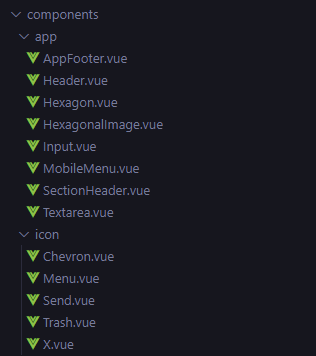
\includegraphics[width=0.25\linewidth]{img/components-structure.png} 
\end{center}
\captionof{figure}{Components implemented}


\section{Extra modules}
List of extra modules imported (pinia, supabase, vuetify) in the project and how they were used

% TODO Non-mandatory staff
\section{Extra functionalities implemented}
Store, Filters, etc

\section{Different approaches}
Different approaches from what was discussed during lectures

\section{SEO and Accessibility}
approaches used to comply with accessibility and SEO guidelines

Accessibility is a fundamental aspect of Web Development and Design and we cared about making our
website as inclusive as possible. For this reason we referenced the WCAG (Web Content Accessibility Guidelines) basic principles and rules 
as early as the User Interface Design stage. 

\begin{center}
    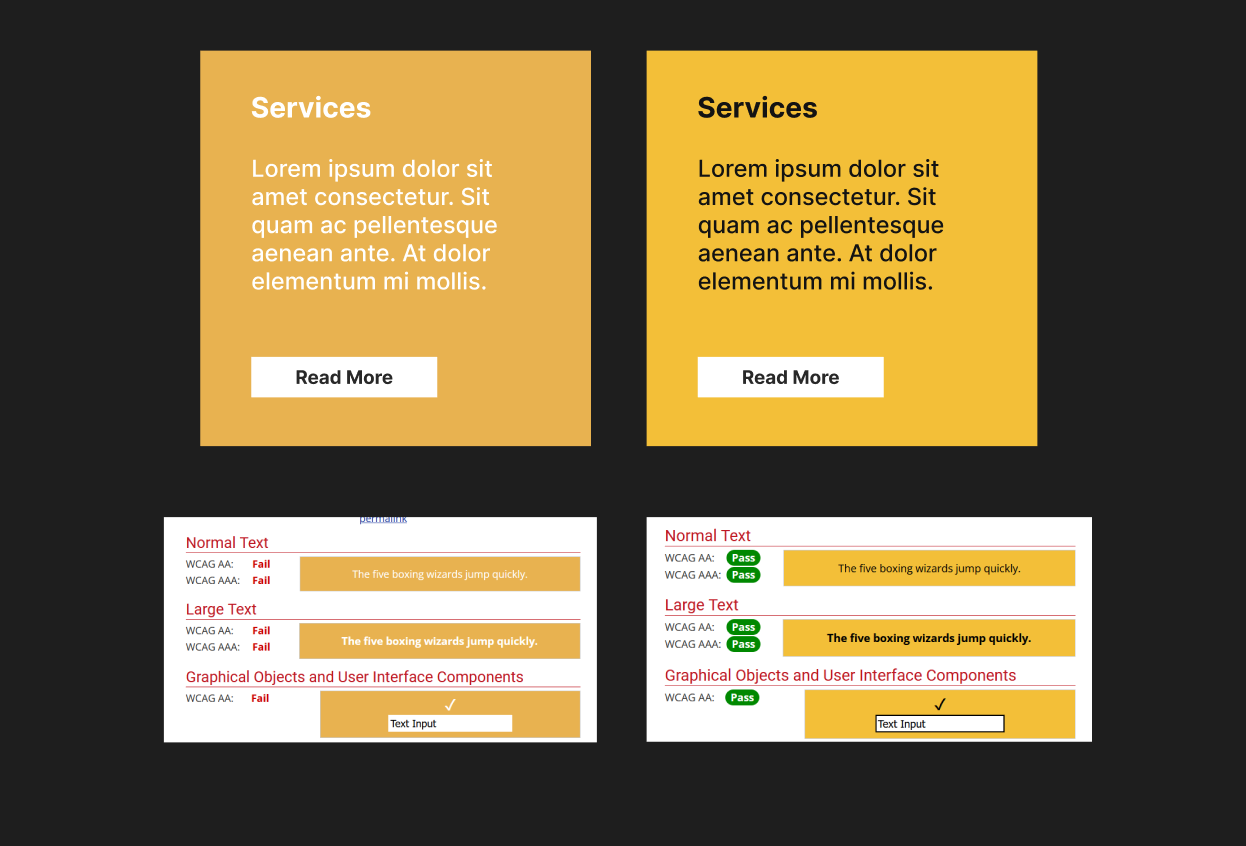
\includegraphics[width=0.75\linewidth]{img/color-contrast-check.png} 
\end{center}
\captionof{figure}{Comparison between early design and newest version}

\vspace{1em}
We mainly focused on color-contrast, alternate-text for images and aria-labels for interactable elements. 
We utilized the tools 'WAVE' and 'Lighthouse' in order to check for possible issues and to calibrate better our
implementation as to increase accessibility, especially for the main functionalities of our website.
This perspective allowed us to also increase by extension the general usability.
Of course these tools are extremely useful but not perfect, and we took care of limit cases by using common sense.
\vspace{1em}

\begin{center}
    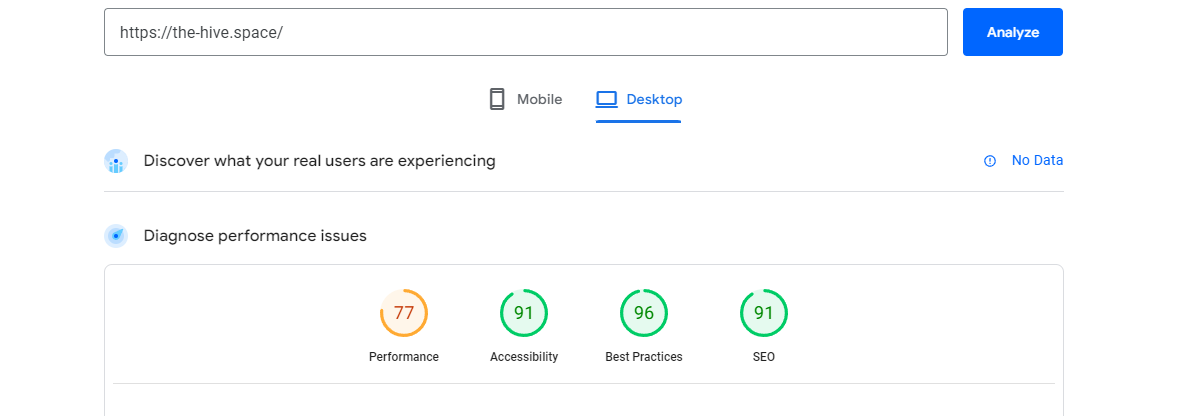
\includegraphics[width=0.75\linewidth]{img/lighthouse-result.png} 
\end{center}
\captionof{figure}{Lighthouse analysis result of the homepage}

\vspace{1em}

\begin{center}
    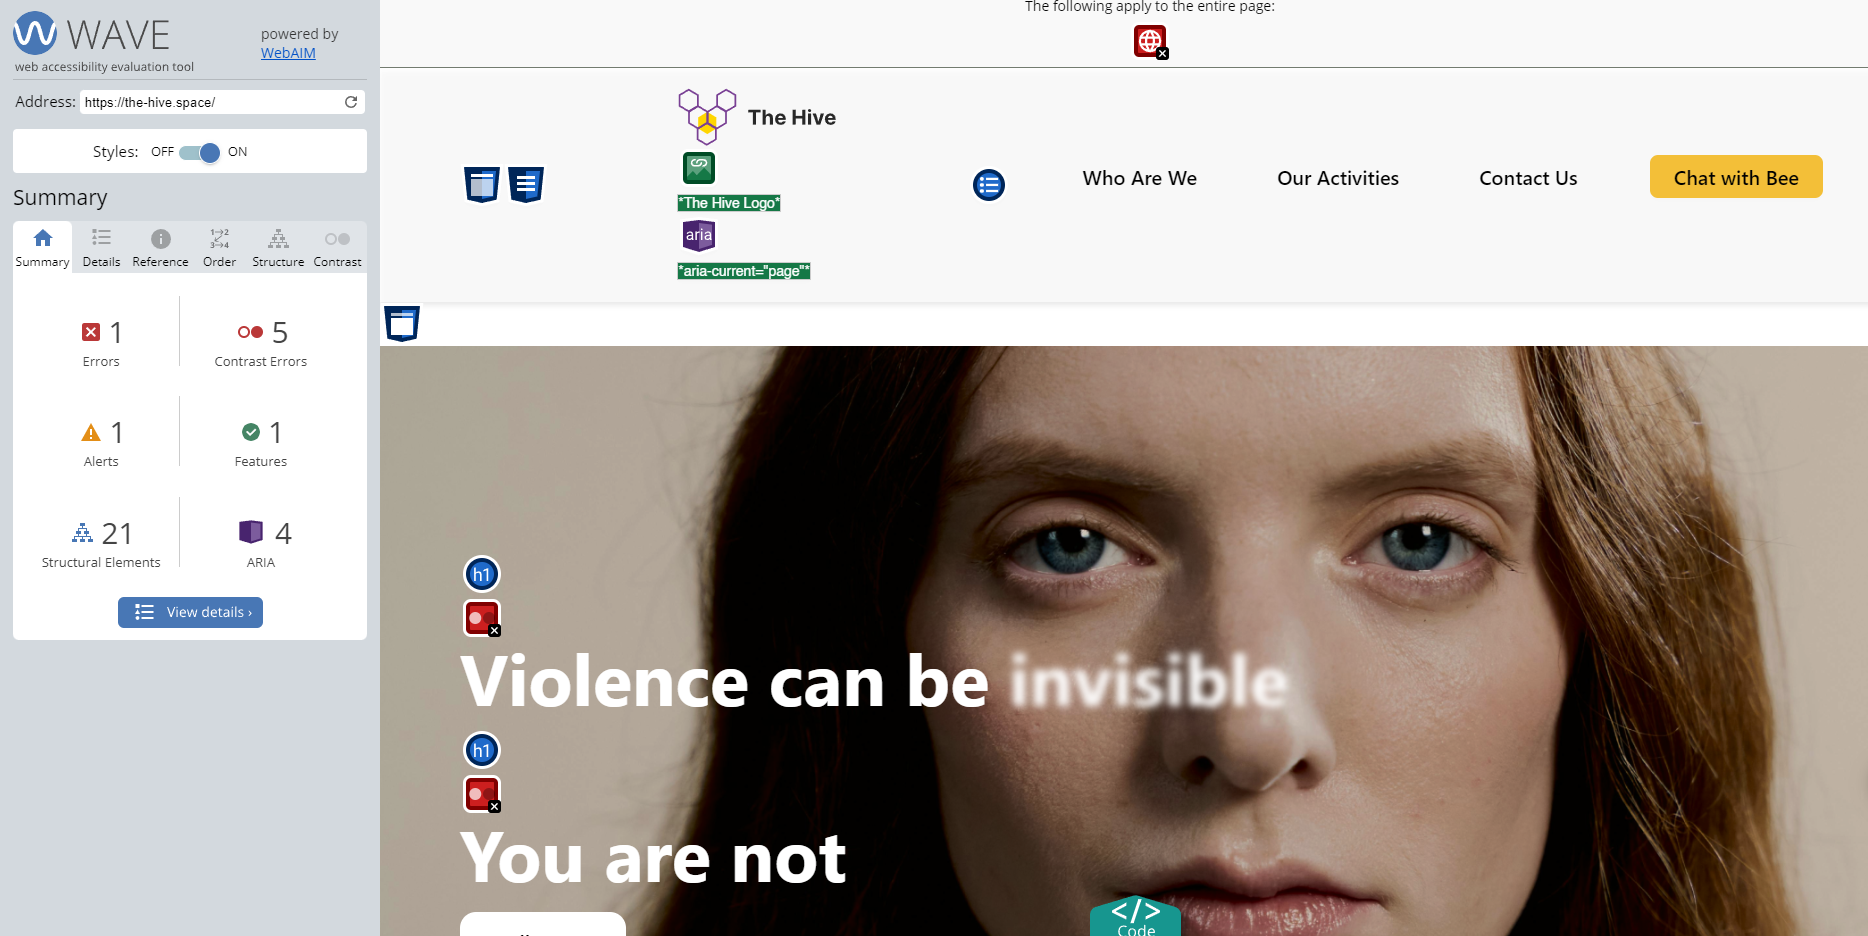
\includegraphics[width=0.75\linewidth]{img/wave-result.png} 
\end{center}
\captionof{figure}{WAVE analysis result of the homepage}
